This layer is responsible for the overall propulsion of the Turing Board. An Electronic Speed Controller (ESC) will be used to regulate the speed of the motor, reverse direction of the motor, and provide regenerative braking. While in autonomous mode the longboard is not capable of using weight to compress the bushing that turn the board. A mechanism is needed that will sit between the trucks and the board that will allow the front truck to rotate independently. This mechanism will be held in place by two solenoids acting as locking pins. A stepper motor using an optical sensor for positioning will interact with gears on the mechanism to rotate it to the desired angle.






\subsection{Electronic Speed Controller}
The electronic speed controller is an electronics circuit that controls and regulates the speed of the motor. The ESC receives desired speed commands from the Jetson TX2 using the CAN bus. Two brushless DC motors, which are embedded into the wheels of the longboard, provide feedback concerning the wheels' direction back to the ESC using hall effect sensors. Using information from both of these systems, the ESC is able to provide current to the motors in order to drive a load at a set speed.


\begin{figure}[h!]
	\centering
 	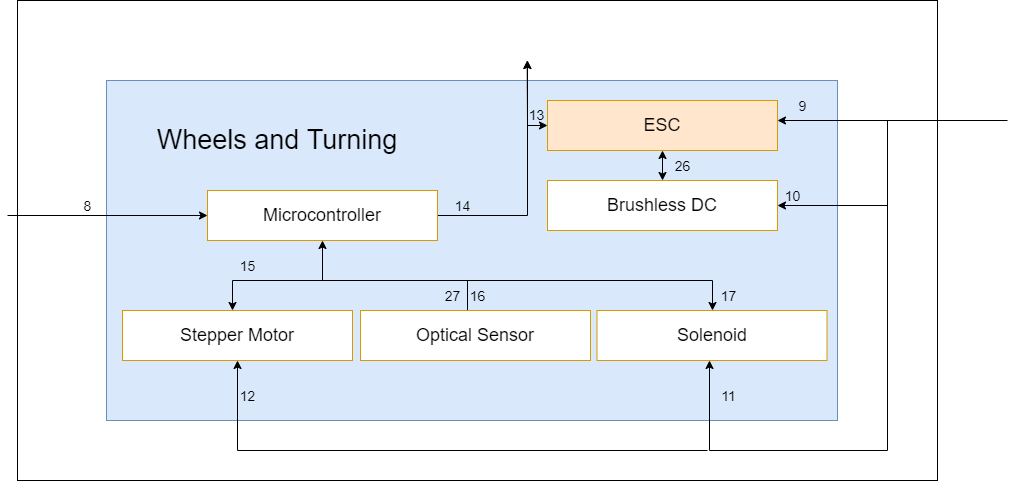
\includegraphics[width=0.60\textwidth]{ADS Latex/images/Keaton/ESC.png}
 \caption{Electronic Speed Controller}
\end{figure}

\subsubsection{Assumptions}
It is assumed that this layer is only called when the board is in use. A speed command must be sent by either the user or the autonomous software.

\subsubsection{Responsibilities}
The ESC is responsible for driving the motor at a constant speed determined by the user. It is also responsible for reversing the direction of the motors to move the longboard backwards if desired. When the brake is applied, the ESC uses its circuitry to redirect the rotational energy of the wheel and recharge the battery powering the longboard.

\subsubsection{Subsystem Interfaces}
Each of the inputs and outputs for the subsystem are defined here.

\begin {table}[H]
\caption {Subsystem interfaces}
\begin{center}
    \begin{tabular}{ | p{1cm} | p{6cm} | p{3cm} | p{3cm} |}
    \hline
    ID & Description & Inputs & Outputs \\ \hline
    \#xx & CAN Bus to Jetson & \pbox{3cm}{Desired Speed} & \pbox{3cm}{Motor RPM}  \\ \hline
    \#xx & Direct Connection to Motor & \pbox{3cm}{Hall Effect Sensor} & \pbox{3cm}{Current to
    Motor}  \\ \hline
    \end{tabular}
\end{center}
\end{table}










\subsection{Brushless DC Motor}
There are two brushless DC motors embedded into the wheels of the longboard. Each motor has three hall effect sensors that allow the speed controller to know how fast the wheels are moving.


\begin{figure}[h!]
	\centering
 	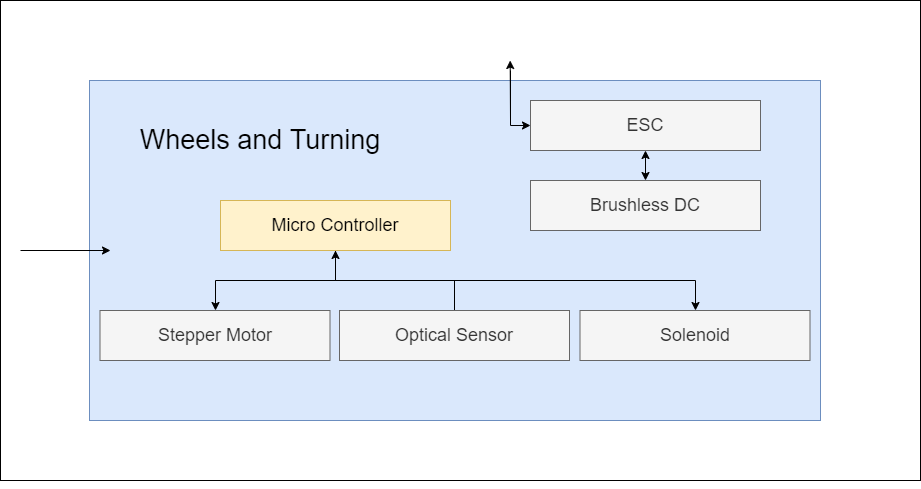
\includegraphics[width=0.60\textwidth]{ADS Latex/images/Keaton/BLDC.png}
 \caption{Brushless DC Motor}
\end{figure}

\subsubsection{Assumptions}
It is assumed that the battery will have sufficient charge in order to power the motor and allow it to rotate.

\subsubsection{Responsibilities}
Rotate when current is applied to the three phases.

\subsubsection{Subsystem Interfaces}
Each of the inputs and outputs for the subsystem are defined here.

\begin {table}[H]
\caption {Subsystem interfaces}
\begin{center}
    \begin{tabular}{ | p{1cm} | p{6cm} | p{3cm} | p{3cm} |}
    \hline
    ID & Description & Inputs & Outputs \\ \hline
    \#xx & Connection to Motor & \pbox{3cm}{Electrical Current} & \pbox{3cm}{Motor Position}  \\ \hline
    \end{tabular}
\end{center}
\end{table}








\subsection{Micro Controller}
The micro-controller will handle the majority of the lower hardware functions such as sensors, solenoids, stepper motor, and PWM control. It will interface with the Jetson TX2.


\begin{figure}[h!]
	\centering
 	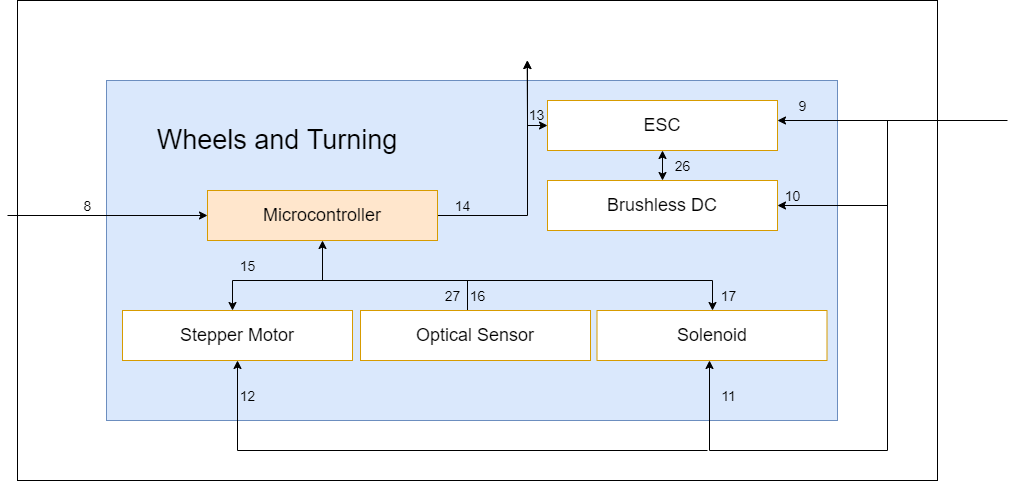
\includegraphics[width=0.60\textwidth]{ADS Latex/images/Keaton/MicroC.png}
 \caption{Micro Controller}
\end{figure}

\subsubsection{Assumptions}
It is assumed that the micro-controller will be receiving constant instructions from the Jetson TX2.

\subsubsection{Responsibilities}
The micro-controller is responsible for direct control of the stepper motor, solenoids, and optical sensors, as well as the corresponding data from each. It is primarily needed to ensure that the turning mechanism is working as intended and will alert the Jetson of any faults that occur.

\subsubsection{Subsystem Interfaces}
Each of the inputs and outputs for the subsystem are defined here.

\begin {table}[H]
\caption {Subsystem interfaces}
\begin{center}
    \begin{tabular}{ | p{1cm} | p{6cm} | p{3cm} | p{3cm} |}
    \hline
    ID & Description & Inputs & Outputs \\ \hline
    \#xx & Connection to Jetson & \pbox{3cm}{Instructions} & \pbox{3cm}{Status Update}  \\ \hline
    \#xx & Optical Sensor & \pbox{3cm}{Motor Position} & \pbox{3cm}{N/A}  \\ \hline
    \#xx & Optical Sensor & \pbox{3cm}{Solenoid Position} & \pbox{3cm}{N/A}  \\ \hline
    \end{tabular}
\end{center}
\end{table}





\subsection{Optical Sensors}
Several optical sensors will be operating in the project. Stepper motors have no method for determining position, but by attaching a piece of metal to the motor we can determine the gear position when the rotating metal breaks the beam of light inside the optical sensor. They will also be used to detect when the plunger of the solenoid has been engaged, blocking the light of the sensor


\begin{figure}[h!]
	\centering
 	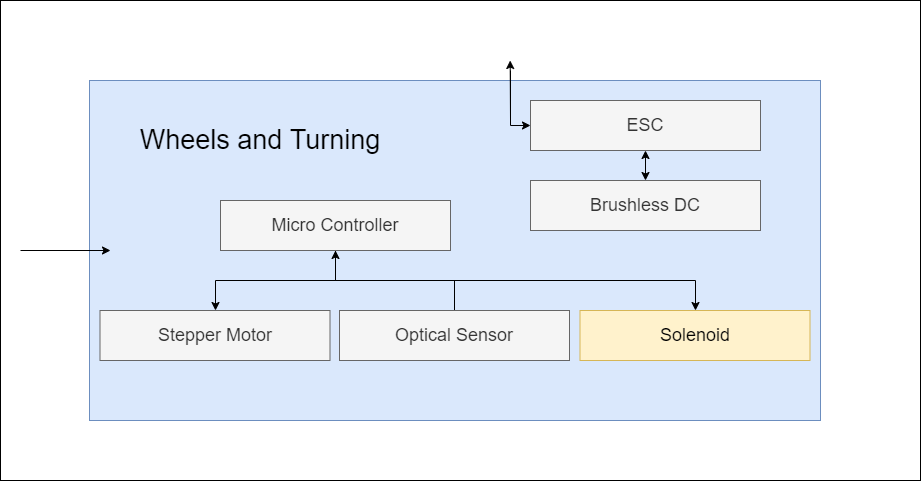
\includegraphics[width=0.60\textwidth]{ADS Latex/images/Keaton/optical.png}
 \caption{Optical sensors will be used for two separate functions}
\end{figure}

\subsubsection{Assumptions}
It is assumed that the sensor will be free of all dirt, debris or any other obstruction that could give false readings to the micro-controller.

\subsubsection{Responsibilities}
Providing the micro-controller information on the stepper motor position or if the solenoids have been engaged.

\subsubsection{Subsystem Interfaces}
Each of the inputs and outputs for the subsystem are defined here.

\begin {table}[H]
\caption {Subsystem interfaces}
\begin{center}
    \begin{tabular}{ | p{1cm} | p{6cm} | p{3cm} | p{3cm} |}
    \hline
    ID & Description & Inputs & Outputs \\ \hline
    \#xx & Connection to Motor & \pbox{3cm}{Motor Shaft} & \pbox{3cm}{Motor Position}  \\ \hline
    \#xx & Connection to Motor & \pbox{3cm}{Solenoid Plunger} & \pbox{3cm}{Solenoid Engaged}  \\ \hline
    \end{tabular}
\end{center}
\end{table}




\subsection{Stepper Motor}
One stepper motor will be utilized to drive a bevel gear that interacts with the turning mechanism. This stepper motor will interface with the micro-controller and will know its position based on an optical sensor mounted on it.


\begin{figure}[h!]
	\centering
 	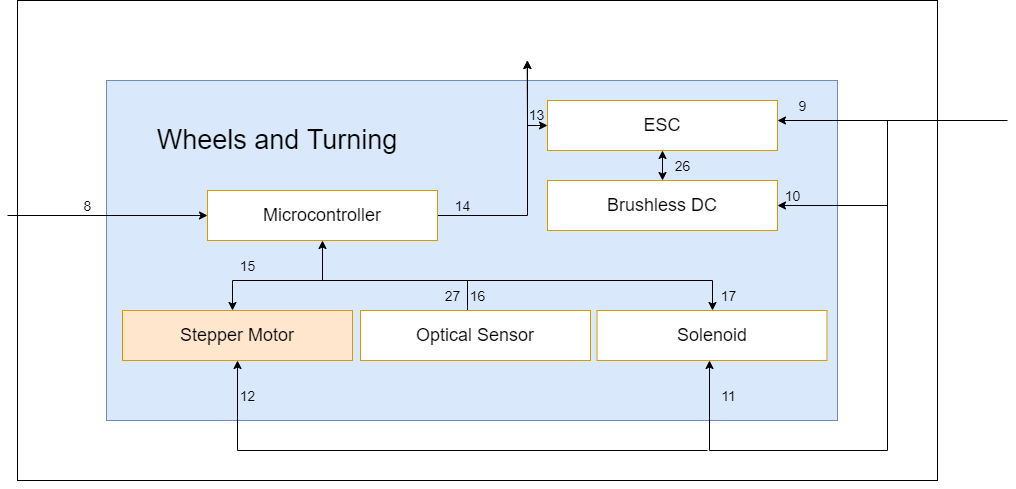
\includegraphics[width=0.60\textwidth]{ADS Latex/images/Keaton/Stepper.png}
 \caption{Stepper Motor}
\end{figure}

\subsubsection{Assumptions}
It is assumed that the optical sensor is operating correctly and relaying the appropriate positional information to the micro-controller

\subsubsection{Responsibilities}
Drive the bevel gear connected to the turning mechanism which allows the trucks to turn.

\subsubsection{Subsystem Interfaces}
Each of the inputs and outputs for the subsystem are defined here.

\begin {table}[H]
\caption {Subsystem interfaces}
\begin{center}
    \begin{tabular}{ | p{1cm} | p{6cm} | p{3cm} | p{3cm} |}
    \hline
    ID & Description & Inputs & Outputs \\ \hline
    \#xx & Connection to Micro-Controller & \pbox{3cm}{Electrical Current} & \pbox{3cm}{N/A}  \\ \hline
    \end{tabular}
\end{center}
\end{table}



\subsection{Solenoid}
A minimum of two solenoids will be utilized as locking pins on the turning mechanism. When needing to turn while the board is in autonomous mode, the code will engage the solenoids to pull them out of the turning mechanism housing. The solenoids will remain engaged while the stepper motor is operational. When turning is complete, the solenoids will be discharged to allow them to return to their position inside the turning mechanism.


\begin{figure}[h!]
	\centering
 	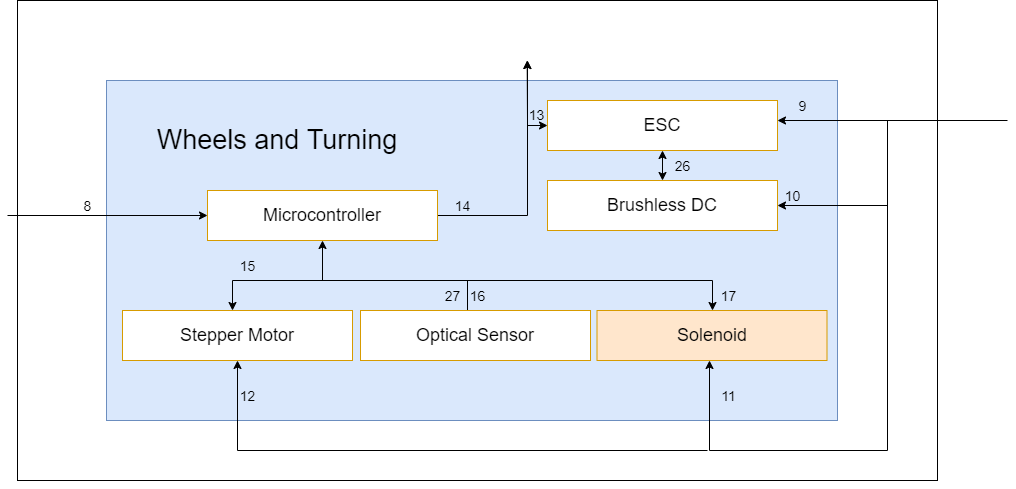
\includegraphics[width=0.60\textwidth]{ADS Latex/images/Keaton/Solenoid.png}
 \caption{Two solenoids will act as holding pins for the turning mechanism}
\end{figure}

\subsubsection{Assumptions}
Solenoids will only engage when in autonomous mode and the truck needs to be able to rotate freely. Optical sensors will be used in conjunction and it is assumed that the micro-controller will always know if the solenoid is engaged or not.

\subsubsection{Responsibilities}
Insert plunger into the turning mechanism when it is at 0 degrees. Prevent the front truck from rotating while in rider mode.

\subsubsection{Subsystem Interfaces}
Each of the inputs and outputs for the subsystem are defined here. 

\begin {table}[H]
\caption {Subsystem interfaces} 
\begin{center}
    \begin{tabular}{ | p{1cm} | p{6cm} | p{3cm} | p{3cm} |}
    \hline
    ID & Description & Inputs & Outputs \\ \hline
    \#xx & Connection to Micro-Controller & \pbox{3cm}{Current} & \pbox{3cm}{N/A}  \\ \hline
    \end{tabular}
\end{center}
\end{table}